\PassOptionsToPackage{bookmarks=false}{hyperref}
\documentclass[conference,final,]{IEEEtran}
\usepackage[bookmarks=false]{hyperref}

\hypersetup{
            pdftitle={A Robust Goal Programming Model With Satisfaction Function For Transfer Pricing Risk Hedging},
            pdfborder={0 0 0},
            breaklinks=true}
\urlstyle{same}  % don't use monospace font for urls

\setcounter{secnumdepth}{0}

\usepackage{graphicx}
\usepackage{amsmath,mathtools}
\usepackage{tikz}
\usepackage{amsfonts}
\usepackage{cite}
\usepackage{booktabs}
\usepackage{pgfplots}
\usepackage{drawstack}
\usepackage{pdflscape}

\usetikzlibrary{shapes.geometric, arrows}
\tikzset{
  font={\fontsize{6pt}{12}\selectfont}}

\providecommand{\tightlist}{%
  \setlength{\itemsep}{0pt}\setlength{\parskip}{0pt}}

\begin{document}

\title{A Robust Goal Programming Model With Satisfaction Function For Transfer Pricing Risk Hedging}

\author{
\IEEEauthorblockN{1\textsuperscript{st} Marco Repetto}
\IEEEauthorblockA{\textit{Department of} \\
\textit{Economics, Management and Statistics}\\
\textit{University of Milan-Bicocca}\\
Milan, Italy\\
m.repetto1@campus.unimib.it}
\and
\IEEEauthorblockN{2\textsuperscript{nd} Davide La Torre}
\IEEEauthorblockA{\textit{Dubai Business School} \\
\textit{University of Dubai}\\
Dubai, UAE \\
dlatorre@ud.ac.ae}
\textit{and}\\
\IEEEauthorblockA{\textit{Department of Economics,} \\
\textit{Management, and Quantitative Methods} \\
\textit{University of Milan}\\
Milan, Italy \\
davide.latorre@unimi.it}
\and
\IEEEauthorblockN{3\textsuperscript{rd} Danilo Liuzzi}
\IEEEauthorblockA{\textit{Department of}\\
\textit{Economics and Management}\\
\textit{University of Cagliari}\\
Cagliari, Italy \\
danilo.liuzzi@unica.it}
}

\maketitle

\begin{abstract}
  In the following paper is proposed a model for controlling the Transfer Pricing risk of a Multinational Firm operating in different countries and that has a well-defined value chain spread across its different controlled companies. These types of agreements controlling such transactions generally take into account different type of objectives. Another problem arises by the process itself that may appear to be fairly deterministic; such simplistic assumption decays if the focus is placed on the general length of such agreements that tend to occupy a medium length planning horizon. Because of that, a Robust Multicriteria Transfer Pricing risk model is built, using the multi-objective capabilities of the Goal Programming approach and the uncertainty modeling features provided by the concept of Robust Optimization. Moreover, the Decision Maker preferences are embedded into the model by leveraging the Weighted Goal Programming approach as well as ad-hoc satisfaction functions for each and every objective. The final result is a model capable of coping with the possible worst-case scenarios in an environment of high uncertainty and mid to long-term planning and robust to scaling.
\end{abstract}

\maketitle

\IEEEpeerreviewmaketitle


\hypertarget{introduction}{%
\section{Introduction}\label{introduction}}
From Apple scandals \cite{leswing18} to Starbucks boycott protests \cite{campbell16} this decade will probably be remembered as the period where the tax avoidance problem gained particular momentum among the people, making the Transfer Pricing (TP) one of the most popular and at the same time most questioned approach. Newspapers and documentaries have spoken massively about this approach, and the fraudulent use that quite a few multinationals have made during these years in order to cut on their tax burden. Most of the time, however, these analyses were inaccurate and somewhat simplistic. Such interest has been shown also by scholars, and it can be quite well inferred by the number of keywords occurrences per year that has been found on the papers indexed by Google Scholar. Figure \ref{keywords} shows clearly that the interest peaked around 2010 when OECD published the first guidelines \cite{oecd10} and remained indicatively constant till nowadays. Still, the number almost doubled since the 00s'. It's not enough to stress the fact that transfer pricing it's just a practice and not a bad one per se \cite{oecd15}. In fact, its aim is to enforce a certain discipline on the transactions involving related parties that otherwise would be settled either arbitrarily or, in the worst case scenario, demanded by tax authorities. Such an alternative perspective on the transfer pricing practice has been also highlighted by recent studies \cite{klassen16}: most of the time, as reported, the goal of the Decision Maker (DM) is not to set a tax scheme in order to achieve overall tax minimization but, on the contrary, the focus is on compliance and, in doing so, controlling the tax risk associated with it. In other words, the rationale is to avoid possible litigation with the tax authorities that can pose at high risk the pricing and possible reserves. Because the risk associated with TP practices is not something affecting solely the companies but also the Tax Authorities, in recent years the OECD addressed this problem and shed some light on the agents operating in such environment \cite{oecd12}, setting some best practices and sharing some evidences given by virtuous countries. Still, even though such contribution are precious for the insights they give, transfer pricing is more than ever as far as possible from being an exact science. Looking at the reference literature very few improvements have been made to model the risk exposure in a rigorous and analytic way. Therefore, the model proposed in this paper tries to embed the expertise made by scholars in the field of Multiple Objective Programming (MOP) and proposes a model for addressing the possible TP risk affecting a multinational company. The aim of this paper is to create a model that gives the Decision Maker (DM) the opportunity to test for a solution that is robust \cite{bertsimas03} and that will guarantee a solution not based only on the evidence of the environment "as-is" but also to a possible worst scenario "to-be". The framework proposed is, therefore, to be considered as a good starting point to a possible intention to review old and deterministic based pricing schemes that do not take into account any possible shifts in the economic environment. Moreover, the overall tastes of the DM are embedded by means of weighting and objective specific satisfaction functions \cite{martel96}.

This paper is divided into three sections. The first deals with the method used to build the model, \emph{i.e.} Goal Programming (GP), Robust Optimization (RO). The second section presents the mathematical formulation of the deterministic model. After that, a possible robust counterpart is suggested where DM preferences are embedded by means of satisfaction functions. In order to solve the model, its mathematical formulation has been coded using the JuMP library\footnote{By the time the article was written version 0.19.0 of JuMP was released, for dependencies issues with minor libraries, version 0.18.0 was used.} \cite{dunning17}\cite{lubin15} of the Julia language \cite{bezanson17} and the solver back-ends chosen were: GLPK, COIN-OR \cite{heimer2003}, IPOPT \cite{waechter05}. In conclusion a brief discussion about possible implementations by multinational firms in their compliance work-flow is given.

\begin{figure}[]
\centering
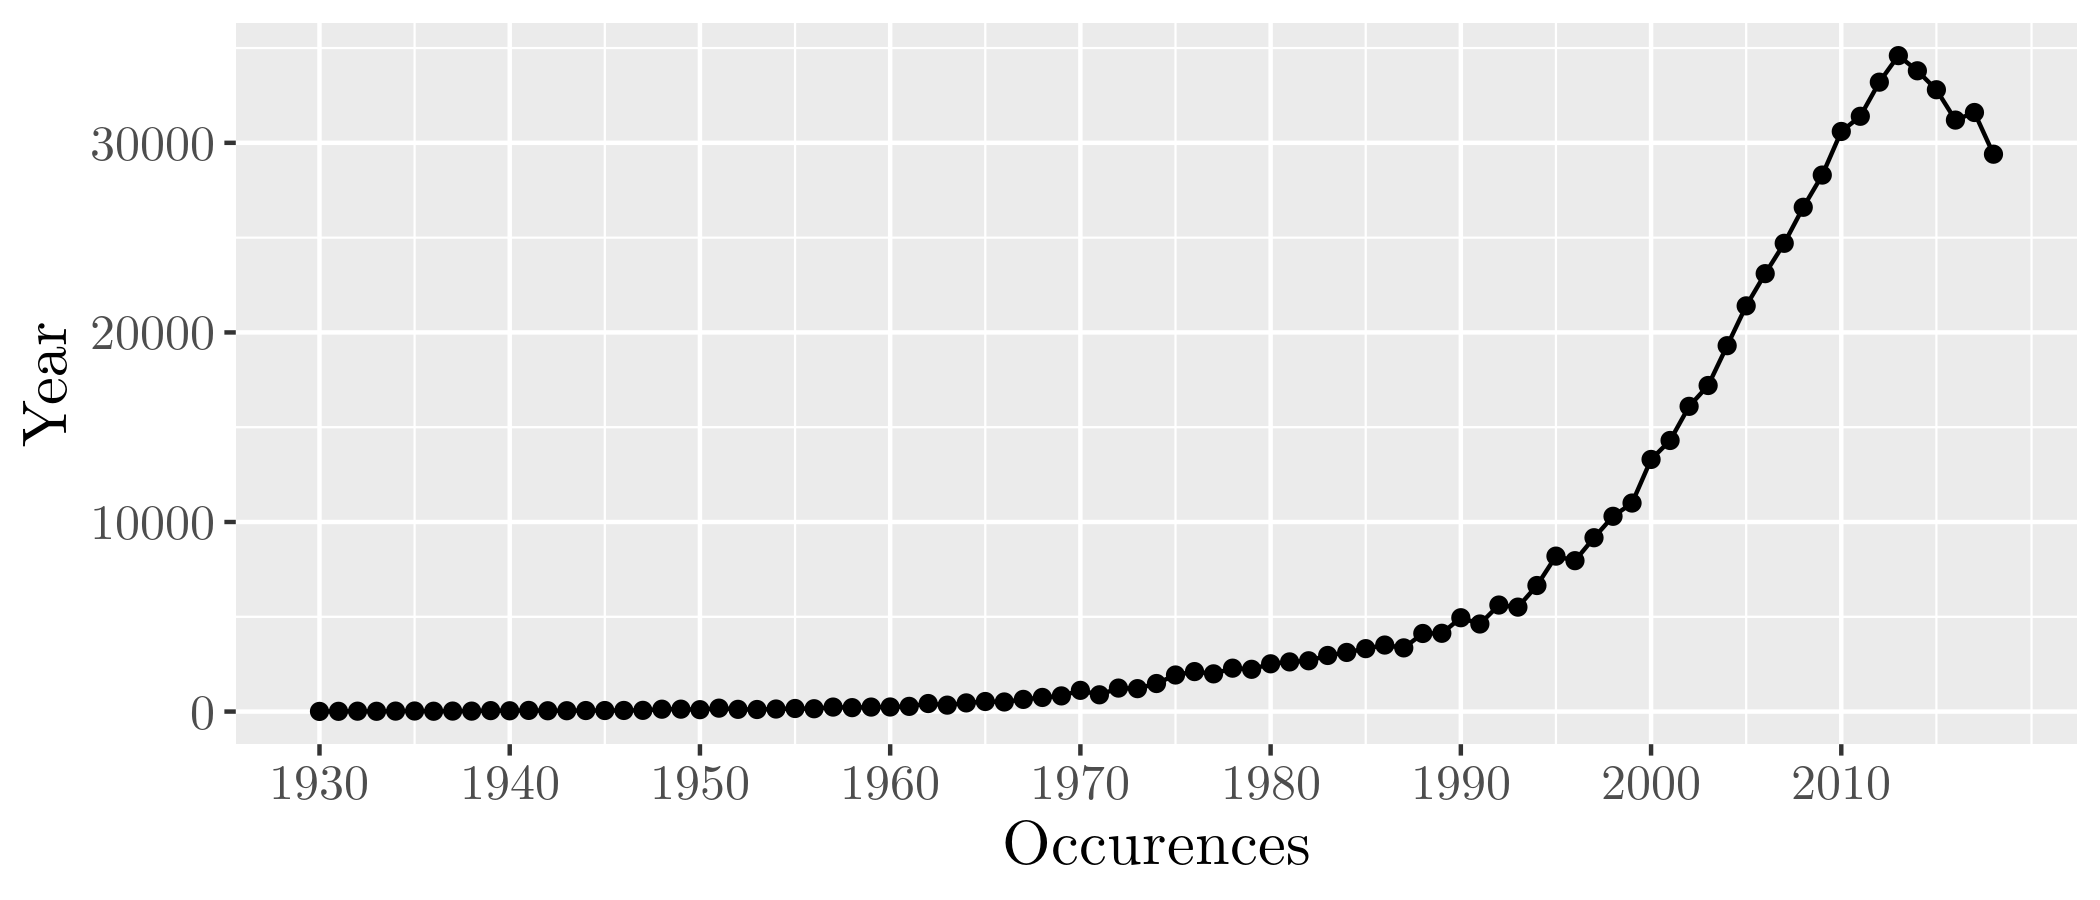
\includegraphics[width=0.45\textwidth]{figure/fig1-1}
\caption{Keyword occurrences per year.}
\label{keywords}
\end{figure}

\hypertarget{methods-used}{%
  \section{Methods used}\label{methods-used}}
This section aims at explaining the main building blocks of model presented in the next section, such building blocks are:
\begin{itemize}
\item Weighted Goal Programming where Gaussian type satisfaction functions were used in order to allow for consistent scaling; 
\item Robust Optimization in its Multi Criteria formulation where the different scenarios where embedded using parametric forms.  
\end{itemize}

\hypertarget{goal-programming}{%
\subsection{Goal Programming}\label{goal-programming}}
The Goal Programming \cite{charnes55} pertains to the field of Multicriteria Decision Analysis (MCDA). MCDA aims at finding a solution that does not look for a single specific goal to be minimized or maximized. Instead, it focuses with problems that carry with them a series of objectives. The rationale behind this approach is very simple. Most of the times decisions problems have different conflicting objectives and the DM has to take into account such additional complexity instead of focusing myopically on a single objective. Goal programming is a distance-based method that relies on minimizing a set of deviation variables which model the distance between achieved levels and goals. In this setting the DM can take into account the deviation of each objective from its goal, and using some projection algorithms the DM can determine Pareto optimal solutions. There are a number of different variants of GP that range from Lexicographic, where the priority of each object is defined a priori, to Min-Max, where the goal focuses on minimizing the maximal deviations from the goals. In this paper, the choice was to use the Weighted Goal Programming (WGP), because it allows for major trade-offs between each and every objective. Its formulation will be generalized and explained in the further paragraph.
\begin{subequations}
The WGP formulation reads as following:
\begin{align}
    & \underset{\{\delta^+,\delta^-\}^N_1}{\text{minimize}} & & \sum^N_{i=1}w_i (\delta^+_i + \delta^-_i) \label{wgpmin} \\
    & \text{subject to} & & f_i(x) - \delta^+_i + \delta^-_i=b_i, \; \forall i \in N \label{wgpsoftgoal} \\
    & & & x\in F \label{wgphardgoal}\\
    & & & \delta^+_i\geq 0, \quad \delta^-_i\geq 0 \quad \forall i \in N \label{wgppositivity}
\end{align}
\end{subequations}
where the objective function in (\ref{wgpmin}) is based on the minimization of the deviations that measure the distance between the objectives and the goals stated in (\ref{wgpsoftgoal}). Equation (\ref{wgphardgoal}) models the presence of more abstract constraints. Such formulation although its versatility has a major drawback, namely the implicit weighting of the objectives given by the different measurement, in other word this type of GP model is scale subjective, this problem, fully addressed by Martel and Aouni \cite{martel96} was partially solved by the use of satisfaction function à là Preference Ranking Organization Method for Enrichment Evaluation (PROMETHEE). Many types of satisfaction function have been suggested by the literature, in this paper the choice was on the following formulation:
$$
F(\delta) = e^{-\frac{\delta^2}{2\sigma^2}}
$$
also called Gaussian satisfaction function which attains it most favorable value when deviations are 0, in Figure \ref{s-function} different parametrization of the $\sigma$ parameter are compared.
\begin{subequations}
The WGP formulation with satisfaction function reads as:
\begin{align}
    & \underset{\{\delta^+,\delta^-\}^N_1}{\text{maximize}} & & \sum^N_{i=1}w_i F_i(\delta^+_i + \delta^-_i) \label{fwgpmin} \\
    & \text{subject to} & & f_i(x) - \delta^+_i + \delta^-_i=b_i, \; \forall i \in N \label{fwgpsoftgoal} \\
    & & & x\in F \label{fwgphardgoal}\\
    & & & \delta^+_i\geq 0, \quad \delta^-_i\geq 0 \quad \forall i \in N \label{fwgppositivity}
\end{align}
\end{subequations}
clearly in this setting the minimization program becomes a maximization one and the objective function becomes non-linear implying either some linearization techniques or the use of different routines capable of handling non-linear optimization problems.
\begin{figure}[]
\centering
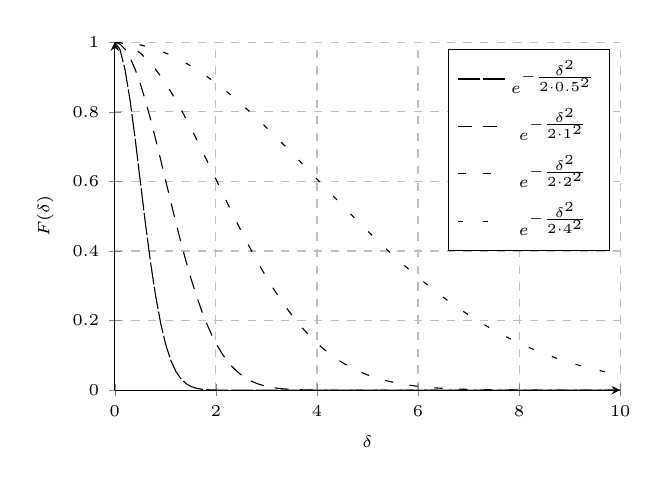
\begin{tikzpicture}
  \begin{axis}[
    width=8cm,height=6cm,
    axis lines = left,
    xlabel = $\delta$,
    ylabel = {$F(\delta)$},
    ymajorgrids=true,
    xmajorgrids=true,
    grid style = dashed,
]

\addplot [
    domain=0:10, 
    samples=100, 
    color=black,
    style= {color=black, dash pattern=on 8pt off 1pt}
]
{exp(-(x^2)/(2*0.5^2)};
\addlegendentry{$e^{-\frac{\delta^2}{2\cdot0.5^2}}$}

\addplot [
    domain=0:10, 
    samples=100, 
    color=black,
    style= {color=black, dash pattern=on 5pt off 4pt}
]
{exp(-(x^2)/(2*1^2)};
\addlegendentry{$e^{-\frac{\delta^2}{2\cdot1^2}}$}

\addplot [
    domain=0:10, 
    samples=100, 
    color=black,
    style= {color=black, dash pattern=on 3pt off 6pt}
    ]
    {exp(-(x^2)/(2*2^2)};
\addlegendentry{$e^{-\frac{\delta^2}{2\cdot2^2}}$}

\addplot [
    domain=0:10, 
    samples=100, 
    color=black,
    style= {color=black, dash pattern=on 2pt off 7pt}
    ]
    {exp(-(x^2)/(2*4^2)};
\addlegendentry{$e^{-\frac{\delta^2}{2\cdot4^2}}$}
\end{axis}
\end{tikzpicture}
\caption{Different Gaussian satisfaction function parametrization.}
\label{s-function}
\end{figure}

\hypertarget{robust-optimization}{%
\subsection{Robust Optimization}\label{robust-optimization}}
It is worth noticing that the classical WGP approach even embedding a satisfaction function does not leave any room for any kind of uncertainty associated with both the coefficients and the goals. These kinds of scenarios are better handled by another type of approach called Robust Optimization. RO builds on the philosophy worst-case analysis and such idea has been applied extensively in many fields, ranging from statistics \cite{huber64} to machine learning \cite{vapnik63}\cite{tibshirani96}. Accounting for uncertainty of parameters in operational research revealed to be crucial in order to avoid sub-optimal solutions or even unfeasible ones \cite{ben-tal00}. In contrast with Stochastic Programming \cite{dantzig55} which assumes probabilistic modeling of the uncertainty; RO reject this assumption posing that parameters vary arbitrarily in known bounded sets, called the uncertainty sets \cite{soyster73}. RO gained momentum in recent years thanks to the extended work of Ben-Tan and Nemirovski \cite{ben-tal97}\cite{ben-tal98}\cite{ben-tal99}.
\begin{subequations}
The robust formulation of the general linear programming model reads as:
\begin{align}
    & \underset{x}{\text{minimize}} & & f(x) \label{rpmin} \\
    & \text{subject to} & & g(x)=\chi(\xi), \; \xi \in \Xi \label{rpcon}
\end{align}
\end{subequations}
where in this case the single goal minimizes the cost function $f(x)$ depending upon the decision variable $x$, given a set of feasible uncertainty regions denoted by $\chi(\xi)$. Here the concept of uncertainty sets, denoted by $\Xi$, is extended to embed an area in which the DM will find its optimal solution. Of course, the feasible uncertainty region can be $N$, where $N=1...+\infty$. In this approach, the more the $N$ we consider the stricter becomes our solution. That's why the RO approach is said to be "conservative", even though in some case it may turn out to be not conservative at all when compared with Stochastic Optimization \cite{ben-tal09}. The figure is an example of how an uncertainty sets might look like. In this case, the picture shows the graphical representation of a bi-dimensional uncertainty set \(\Xi\) which has to be compact and convex. Each element \(\xi_i\) of \(\Xi\) corresponds to a feasible region defined by \(\chi(\xi)\). The RO problem shown above has two major drawbacks, namely: (i) it does not include any measure of robustness which the DM can act on, and (ii) it does not allow (by design) to consider multiple objectives. A hybrid approach that tries to fix both of these problems affecting early stage RO formulations was originally developed by Kuchta \cite{kuchta04}. In this formulation, the robust tuning parameter is played by \(r\) where \(r=0...n\) given \(n\) the number of parameters subjected to uncertainty.
\begin{subequations}
The compact formulation of a robust goal programming model reads as:
\begin{align}
    & \underset{\{\delta^+,\delta^-\}^N_1}{\text{minimize}} & & \sum^N_{i=1}w_i (\delta^+_i + \delta^-_i)  \label{wrgpmin} \\
    & \text{subject to} & & f_i(x) + \sum_{j=1}^{Q}p_{ij} + r_iz_i - \delta^+_i + \delta^-_i = b_i, \forall i \in N  \label{wrgpsoftgoal} \\
    & & & z_i + p_{ij} \geq g_{ij}(x), \forall i \in N , \forall j \in Q \label{wrgptuning} \\
    & & & x\in F \label{wrgphardgoal} \\
    & & & \delta^+_i,\delta^-_i, p_{ij}, z_i \in \mathbb{R}^{+} \label{wrgppositivity} \\
    & & & x \in \mathbb{R}^{s} \label{wrgpfeasible}
\end{align}
\end{subequations}
The deviations in Equation (\ref{wrgpmin}) are weighted using the function $w$. It is worth noticing that in this formulation the tuning parameter that permits to adapt the level of robustness, sometimes referred to as the price of robustness \cite{bertsimas04} represented by \(r\), whereas Equation (\ref{wrgphardgoal}) models the presence of more abstract constraints. The formulation proposed by Kuchta was used by Ghahtarani and Najafi in the field of portfolio optimization \cite{ghahtarani13} where uncertainty affected the parameters related to portfolio selection resulting in a solution with an increased conservatism as well as its price of robustness.
\begin{figure}[]
\centering
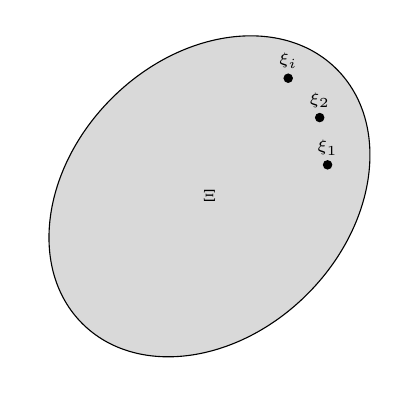
\begin{tikzpicture}
\draw[rotate=-45,fill=gray!30] (0,0) ellipse (50pt and 65pt);
\filldraw (1.5,0.4) circle[radius=1.5pt];
\filldraw (1.4,1)   circle[radius=1.5pt];
\filldraw (1,1.5)   circle[radius=1.5pt];
\node[above] at (1.5,0.4){$\xi_1$};
\node[above] at (1.4,1)  {$\xi_2$};
\node[above] at (1,1.5)  {$\xi_i$};
\node[] at (0,0) {$\Xi$};
\end{tikzpicture}
\caption{Uncertainty set and its elements.}
\label{u-set}
\end{figure}

\hypertarget{the-model}{%
\section{The Model}\label{the-model}}
As stated previously, when dealing with the setting of the transfer prices, the DM faces a series of choices that most of the times conflict with each other, ranging from management profitability requirements to greedy tax minimization, hence a GP model has been chosen. Apart from the number of objectives considered a key role is played by the dynamics of the environment in which such decisions are taken, such environment tends to be influenced by a certain degree of uncertainty, and therefore the TP policies have to be robust in the sense that has to account for that uncertainty. However, before start modeling the uncertainties related to the exogenous variables affecting the decision process, it will be worth enunciating the characteristics underpinning transfer pricing policies, then a full deterministic version of the model will be proposed, after that, the last section is devoted to introducing the robust counterpart of the deterministic model and aim at explaining the possible uncertainties affecting the environment.

\hypertarget{transfer-pricing}{%
\subsection{Transfer Pricing Policies}\label{transfer-pricing}}
As state in the last section, the TP is a particular field of international taxation that deals with the decision on how to set the price among companies belonging to the same group. In order to enact this decision not arbitrarily, some best practices were further developed \cite{oecd17} and in some countries around the world, such practices have been embedded in the legislation. Generally, Multinational Entities (MNE) subject to such legislative burden tend to act proactively promoting agreements that bind the counterparts belonging to the same group for particular value-related process, an example may be given by the value chain process related to the delivery of a produced good to the final customer; in this setting is possible to identify different aspects, namely:
\begin{itemize}
\item The counterparts: are the agents involved in the transaction, generally more than one, in the case under the scope of analysis in this paper the agents were three, namely the manufacturer, the distributor, and the principal entity.
\item The role of the counterparts: are the activities that each agent will perform, the role is crucial in order to determine the policy of remuneration to be applied, in the case under analysis the activities are:
  \begin{itemize}
  \item Production: to produce the good with the specifics imposed by the headquarter or by whom is supposed to enforce such specifics;
  \item Distribution: to distribute the good from the production facility to the retail area, this activities may imply limited marketing and sales force activities;
  \item Principal: to coordinate the production and distribution activities and audit the overall process in order to accomplish the firm's standard, this role implies also the risk management process and risk-bearing activities.
  \end{itemize}
\item The remuneration of the counterparts: the following aspect is strictly connected with the previous point, that is, generally the remuneration is given by the risk exposure of each specific party, in case of a distribution agreement generally the most of the risk is born by the principal because of the role of controller and risk-bearer within the whole value process, however it is worth noting that do not exist a rule of thumb that allocates the risk exposure within every entity part of the agreement.
\item Auxiliary clauses: not in the scope of analysis of the model because merely legal, they may imply aspects such as terms of payments and resolution clauses.
\end{itemize}
The aspect of remuneration is crucial in these policies because may lead tax avoidance conducts. In the best practices provided by the OECD several methods are proposed to cope with this aspect as presented in figure \ref{fig:tp-m}. In the case under analysis we excluded the Traditional Transaction Methods because of a lack of comparable transactions involving the MNE and other third parties unrelated companies, many times such traditional methods imply economic relations with other agents in the market which are not a viable option for highly integrated companies that tend to control the majority of the value chain, and apart from that when it exists such third party transaction the product or good involved may not embody all the characteristics of the product under TP analysis. Therefore, the choice was to opt for Transactional Profit Methods, in such case the relevant information may be obtained by commercial databases who sell financial data related to companies. The Transactional Net Margin Method (TNMM) is based on the examination of the net profit relative to an appropriate base (e.g. costs, sales, assets) that a local entity realizes from a controlled transaction (or in our case to the entity itself). In order to achieve this is necessary to identify which Profit Level Indicator to choose; this is an important choice that has to be made taking into account the functional characterization of such entity, that is, if an entity focuses on distribution the best PLI to test such entity is given by the ROS of its functional characteristics, that's because the sales are supposed to be the main element of a distributor (and not cost or assets). The main PLIs used by the practitioners are: Return on Sales, Full Cost Mark-up, Return on Asset, Return on Investment. After each functional characteristic is matched with its relative PLI it's necessary to find the data of comparable independent entities, in order to asses the profitability range that our entity has to obtain to be in an arm's length position.
\begin{figure*}
\centering
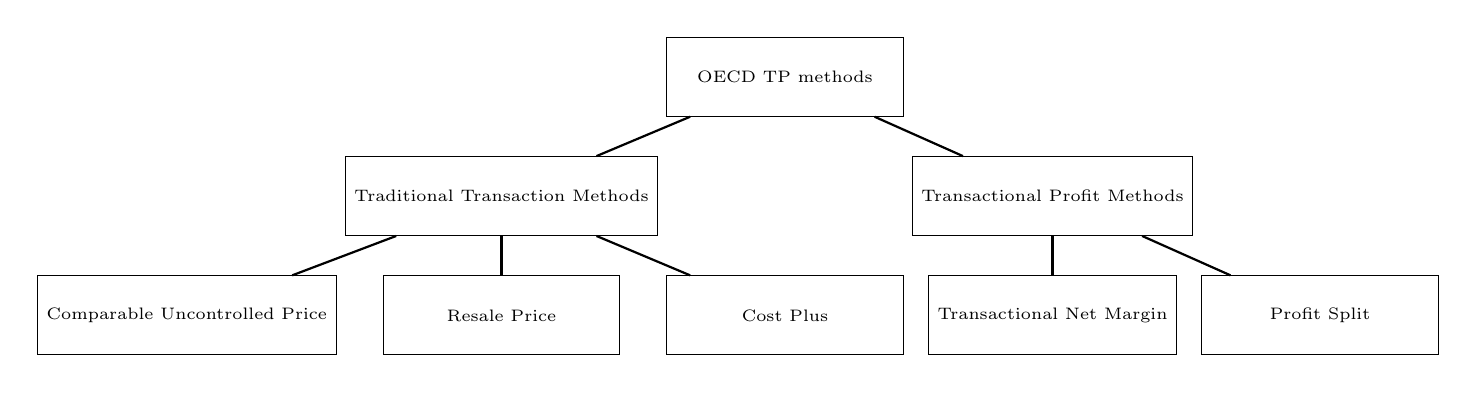
\begin{tikzpicture}
  \matrix [column sep=1mm, row sep=5mm] {
    & &
  \node (yw) [draw, shape=rectangle,minimum height=1cm, minimum width=3cm,align=center] {OECD TP methods}; &
  & \\
  &
   \node (d1) [draw, shape=rectangle,minimum height=1cm, minimum width=3cm,align=center] {Traditional Transaction Methods}; & &
  \node (d2) [draw, shape=rectangle,minimum height=1cm, minimum width=3cm,align=center] {Transactional Profit Methods}; & \\
  \node (we) [draw, shape=rectangle,minimum height=1cm, minimum width=3cm,align=center] {Comparable Uncontrolled Price}; &
  \node (wf) [draw, shape=rectangle,minimum height=1cm, minimum width=3cm,align=center] {Resale Price}; &
  \node (wg) [draw, shape=rectangle,minimum height=1cm, minimum width=3cm,align=center] {Cost Plus}; &
  \node (pu) [draw, shape=rectangle,minimum height=1cm, minimum width=3cm,align=center] {Transactional Net Margin}; &
  \node (pl) [draw, shape=rectangle,minimum height=1cm, minimum width=3cm,align=center] {Profit Split}; \\
};
\draw[-, thick] (d1) -- (we);
\draw[-, thick] (yw) -- (d1);
\draw[-, thick] (yw) -- (d2);
\draw[-, thick] (pu) -- (d2);
\draw[-, thick] (d1) -- (wg);
\draw[-, thick] (d1) -- (wf);
\draw[-, thick] (d2) -- (pl);
\end{tikzpicture}
\caption{TP methods in the OECD guidelines.} \label{fig:tp-m}
\end{figure*}

\hypertarget{deterministic-model}{%
\subsection{Deterministic TP policy model}\label{the-model}}
The model that is going to be presented tries to cope with several objectives coming from different vision of the company that ranges from greedy tax minimization to management profit achievement. Therefore, the model proposed has to:
\begin{enumerate}
\def\labelenumi{\arabic{enumi}.}
\tightlist
\item
  Minimize the Group Tax Liability to a target level decided a priori by
  the management;
\item
  Foster the compliance with each and every functional characterization
  of the Group entity using the TNMM;
\item
  Fulfill the management goals for each division off-shore in terms of
  product margin.
\end{enumerate}
These objectives will constitute the soft constraints subjected to the deviational variables. From the aforementioned objectives some hard constraints will result; in particular from the second objective, namely the one involving TNMM compliance carries with it two types of hard constraints: the first one related to the lower boundary of the profit level indicator that should not fall below the lower quartile of the dataset of comparable profit indicators selected to apply the TNMM, the second hard constraint does the same, providing an upper ceiling of the profit level indicator that mustn't score higher than the upper quartile of the dataset provided to test the arm's length nature of the transaction. An entity failing to comply with such requirement may put at stake its compliance dramatically increasing its tax risk. The last hard constraints will be on product price and do not derive from any of the objectives mentioned above, that is, because of pricing adjustment the final price may be subjected to small increases or decreases but these movements cannot be far to higher because of the competitiveness of the market. In such approach the decision was to fix the remuneration in terms of products delivered therefore the model was a product centric one, this is generally the best practice adopted by practitioner that tend to avoid fixed fees that would force constant revision of the policies. As a consequence all the decision variables are expressed as product's profit margin. The nature of the decision variable to be a net profit margin and not a measure of the revenue is due to the fact that the entities involved have already been decided therefore costs cannot be subjected to any possible allocation. The corresponding algebraic formulation not taking into account any uncertainty related to the data is the following:
\begin{subequations}
Deterministic WGP model formulation:
\begin{align}
    & \underset{\delta^+,\delta^-}{\text{minimize}} & & \sum^{N}_{i=1}w_iF_i(\delta^+_i + \delta^-_i) & \label{dm_obj} \\
    & \text{subject to} & & n\cdot \sum^{Q}_{j=1}(x_j\cdot t_j) - \prescript{t}{}{\delta^+}  =\overset{\star}{t} & \label{dm_tax} \\
    & & & n\cdot \frac{x_j}{b_j} - \prescript{m}{}{\delta^+_j} + \prescript{m}{}{\delta^-_j} = m_j, & \forall j \in Q \label{dm_median} \\
    & & & {x_j} - \prescript{g}{}{\delta^+_j} + \prescript{g}{}{\delta^-_j} = g_j, & \forall j \in Q \label{dm_management} \\
    & & & \sum^{Q}_{j=1} c_j(x_j) \geq p & \label{p_l} \\ 
    & & & \sum^{Q}_{j=1} c_j(x_j) \leq p + \Delta & \label{p_u} \\
    & & & n\cdot \frac{x_j}{b_j} \geq l_j, & \forall j \in Q \label{l_q} \\
    & & & n\cdot \frac{x_j}{b_j} \leq u_j, & \forall j \in Q \label{up_q}\\
    & & & \delta^+_i,\delta^-_i,x_j\geq 0  & \forall i \in N, \quad \forall j \in Q
\end{align}
\end{subequations}
Where the three types of deviational variables (highlighted by \(^t\),\(^m\), \(^g\)) belong to main objectives described below, in particular:
\begin{itemize}
\item Equation (\ref{dm_tax}): refers to the tax minimization, in such objective the goal is to penalize any positive deviation in order to achieve the target tax liability level decide a priori by the management in this case $\overset{\star}{t}$ has to be intended has the absolute value of tax expenses that MNE would like to pay wereas the left-hand side represent the current tax liability identified as:
  $$
  n\cdot \sum^{Q}_{j=1}(x_j\cdot t_j)  = \text{EBIT} \cdot \text{Tax Rate} = \text {Tax Liability} 
  $$
\item Equation (\ref{dm_median}): refers to the TNMM goal for the net profit indicator to be in line with the median of a particular set of independent companies $m_j$ performing similar functions, wereas the left-hand side represent the Earnings Before Interest and Taxes over the applicable base defined by TNMM in other terms:
  $$
  n\cdot \frac{x_j}{b_j} = \frac{\text{EBIT}_j}{\text{BASE}_j} \quad j \in Q \quad b = \begin{bmatrix} \text{Return On Sales} \\ \text{Return On Assets} \\ \vdots \end{bmatrix}
  $$
\item Equations (\ref{l_q}) and (\ref{up_q}): represent the lower and upper quartile indicator boundary of the TNMM, as mentioned above this provide the range in which the tax risk result on a controllable level therefore these two equations are strictly related with the previous one additional reference of such data is provided on the Data Transparency section;
\item Equation (\ref{dm_management}) sets the management's objectives for each off-shore division in terms of margin per product.
\item Equation (\ref{p_l}) and (\ref{p_u}) sets minimum and maximum price deviation accepted because of the TP policy; 
\end{itemize}
As mentioned previously the decision variables \(x\) represent the margin of the product allocated to the j-th firm. In this setting, a particular attention should be given to the base coefficient \(b\) that is divided by the \(x\) margin: this operation results in the net profit level indicator which is necessary to assess the arm's length nature of the transaction involving the companies. In the design of such a model the following simplistic assumption have been taken into account:
\begin{itemize}
\item
  No Value Added Tax has been taken into account, that is, the only tax
  taken into account was the one on corporate income;
\item
  The cost variable takes into account a number of different aspects
  from material to manpower: this simplification allowed for shorter
  formulation of the deterministic model;
\item
  The focus was ultimately on products whereas in many cases it could be
  different. As previously stated the model is product centric but
  ultimately, when the margin is set to the single product, it can be
  fully extended to whatever measure will be used in the policy (they
  may be series of products or even something else).
\end{itemize}
All the following simplifications have been made in order to highlight the main process, and they may be taken apart in case of more practical situations. In the next section is introduced the robust counterpart of such model accounting for the high uncertainty.

\hypertarget{the-robust-counterpart}{%
\subsection{The Robust Counterpart}\label{the-robust-counterpart}}
The model presented above is deterministic, which is a very strong assumption in an environment where exogenous variables might change. We now relax the deterministic assumption and leave some room to the potential uncertainty that may occur. In particular, the robustness of the model was tested against three different factors:
\begin{enumerate}
\def\labelenumi{\arabic{enumi}.}
\tightlist
\item Possible uncertainty about the tax rate;
\item Possible uncertainty about duties;
\item Possible uncertainty regarding the feasible range of compliance with the TNMM.
\end{enumerate}
\begin{subequations}
Robust WGP model formulation:
\begin{align}
& \underset{\delta^+,\delta^-}{\text{minimize}} \sum^{N}_{i=1}w_iF_i(\delta^+_i + \delta^-_i)\\
& \text{subject to} \sum^{Q}_{j=1}(x_j t_j + \pi_{1,j})+ \prescript{t}{}{\rho} \prescript{t}{}{\zeta} - \prescript{t}{}{\delta^+}  =\overset{\star}{t} \\
& n\cdot \frac{x_j}{b_j}+\pi_{2,j}+ \prescript{m}{}{\rho} \prescript{m}{}{\zeta} - \prescript{m}{}{\delta^+} + \prescript{m}{}{\delta^-_j} = {m_j}, & \forall j \in Q \\
& {x_j} - \prescript{g}{}{\delta^+_j} + \prescript{g}{}{\delta^-_j}  = {g_j}, & \forall j \in Q \\
& \sum^{Q}_{j=1} c_j(x_j) + \pi_{3,j} + \prescript{t}{}{\rho} \prescript{g}{}{\zeta} \geq p \\
& \sum^{Q}_{j=1} c_j(x_j) + \pi_{3,j} + \prescript{t}{}{\rho} \prescript{g}{}{\zeta} \leq p + \Delta \\
& n\cdot \frac{x_j}{b_j} \geq {l_{j,u}}, \qquad  \forall j \in Q, \quad \forall u \in U \label{lquartile} \\
& n\cdot \frac{x_j}{b_j} \leq {u_{j,u}}, \qquad \forall j \in Q, \quad \forall u \in U \label{uquartile} \\
& \zeta_i + \pi_{ij} \geq \theta_{ij} x_{j},  \qquad \forall i \in N, \quad \forall j \in Q \\
& \delta^+_i,\delta^-_i,x_j\geq 0, \qquad \forall i \in N, \quad \forall j \in Q
\end{align}
\end{subequations}
In this formulation, we used the approach developed by Kuchta focusing
not only on the soft constraints but also on the hard ones, as in Equations (\ref{lquartile}) and (\ref{uquartile}).

\hypertarget{data transparency}{%
\subsection{Data Transparency}\label{data transparency}}
In populating the model with the data we distinguish two types of it:
\begin{itemize}
\item Internal data: related solely on the company and its subsidiaries, this data may include shipping costs, selling intercompany profit goals and more;
\item External data: related to competitors and on the whole environment where the company operates, a typical external data may be the corporate tax or the revenue achieved by a specific competitor.
\end{itemize}
The internal data provided to the model were collected from a leading company in telecommunications and networking appliances with its production facility based in the Far-East and with the principal and distributional functions based in the European Union soil. Because of a matter of confidentiality, the data were anonymized, with this procedure the relevant functionalities of the model remained intact although preserving the corporate financial strategies. Conversely, the external data used for the TNMM method application were obtained by ad-hoc business related databases such as Orbis \cite{orbis} provided by Bureau van Dijk a major publisher of business information, specialized in private company data. In the following tables is given an overview of such data, starting with the product-oriented goal information which is provided in Table I, whereas the additional goals and data specific of the entities involved in the intercompany value chain are presented in Table II. The noise matrix \(\theta^{Q \times (N\cap N^0) }\) applied to the coefficient was the following one:
\[ \mathbf{\Theta} =  \begin{bmatrix}
 0.0125 & 0.0750 & 0.0060 & 0.0120 & 0.0210 \\
 0.0300 & 0.0000 & 0.0012 & 0.0024 & 0.0060 \\
 0.0250 & 0.0000 & 0.0042 & 0.0147 & 0.0294 \\
 \end{bmatrix} \]
These have to be intended as the maximum shifts that each variable may
be subjected to. In both cases, namely with the corporate taxes and duties,
these shifts may be positive, whereas in case of the TNMM values such
shifts will be negative since a lower level of the test PLI will result
in a worst case scenario and not the other way around.
\begin{table}[]
\centering
\caption{Product specific goal.}
\label{ps-goal}
\begin{tabular}{@{}lll@{}}
\toprule
No. Items    & Price & Tax Goal \\ \midrule
1000000.0 & 61.2  & 0.10    \\ \bottomrule
\end{tabular}
\end{table}
\begin{table*}[]
\centering
\caption{Entity specific data and goals.}
\label{es-goal}
\begin{tabular}{@{}lllllllllll@{}}
\toprule
ID & Function & Tax-Rate   & Variable Cost & Fixed Cost    & Duty & Management Goal & Lower Quartile & Median & Upper Quartile \\ \midrule
1  & manufacturer & 0.25  & 23.75 & 811800.0 & 0.15   & 3.2   & 0.04      & 0.08   & 0.14      \\
2  & distributor  & 0.30  & 11.3  & 35700.0  & 0.0    & 2.8   & 0.01      & 0.02   & 0.05      \\
3  & principal    & 0.125 & 16.8  & 171000.0 & 0.0    & 5.1   & 0.02      & 0.07   & 0.14      \\ \bottomrule
\end{tabular}
\end{table*}

\hypertarget{model-deploy}{%
  \subsection{Model Deploy}\label{model-deploy}}
Model deploy was pursued through Julia\footnote{Version 1.1.0, built on GNU/Linux Fedora 30 Workstation.} as the higher level programming language which provides state-of-the-art interfaces to popular solvers as well as wrappers to top visualization and management tools for data analysis. Julia is a high-level, high-performance dynamic programming language for technical computing. The main feature of Julia is given by its high-performance design, due to the Just In Time (JIT) compiling features it allows for a performance that in some situations resemble the same performance achieved by other low level compiled languages such as C and at the same time maintains a syntax that is readable and focused on the task. The full stack used for the deployment of the model was divided as such:
\begin{itemize}
\item Plotting stack: the plotting functions were achieved by using the main plotting library of Julia that is Plots \cite{plots18} which is a wrapper of several plotting back-ends such as PGFplots and Matplotlib \cite{matplotlib07}, another plotting library used was Gggplot2 \cite{ggplot206} provided by the R package \cite{r18}.
\item Data management stack: the data management process was accomplished by Julia Data framework.
\item Algebraic modeling stack: the formalization of the robust model was obtained by using JuMP, a modeling language for mathematical optimization embedded into Julia and for the implementation of the Lexicographic approach the vOptSolver\cite{xavier17} library was used.
\item Solvers stack: the solver stack was primarily divided into three solvers:
  \begin{itemize}
  \item COIN-OR Linear Programming solver: the interface was provided by the Clp.jl package embedded into the JuliaOpt library;
  \item GNU Linear Programming Kit: the interface was provided by the Julia GLPK module embedded into the JuliaOpt library;
  \item Interior Point Optimizer: the interface was provided by the Julia Ipopt.jl package.
  \end{itemize}
\end{itemize}
In Figure \ref{stack} is proposed a stack diagram highlighting all the building blocks of the process of deployment. The hardware in which the model was deployed had the following specifics:
\begin{itemize}
\item CPU: Intel Core i7-7Y75 CPU at 1.30GHz x 4;
\item RAM: 15,5 GiB;
\item GPU: Intel HD Graphics 615 (Kaby Lake GT2).
\end{itemize}
\begin{figure}[]
\begin{center}{
\tikzstyle{freecell}=[fill=white!10,draw=blue!30!black]
\tikzstyle{occupiedcell}=[fill=white!10!orange!10,draw=blue!30!black]
\tikzstyle{padding}=[fill=white!20,draw=blue!30!black]
\tikzstyle{highlight}=[draw=white!50!black,text=orange!50!black]
\begin{drawstack}
  \cell{PGFplot, Matplotlib, Gggplot2}
  \cell{DataFrames}
  \cell{JuMP,vOptSolver}
  \cell{Julia, R}
  \cell{MathProgBase}
  \cell{COIN-OR LP, GLPK, IPopt}
\end{drawstack}}
\end{center}
\caption{Full Stack chart.}
\label{stack}
\end{figure}

\hypertarget{results}{%
\section{Results}\label{results}}
As deeply specified in the previous section the model was generalized with the Julia Language framework JuMP and the resulting model was solved using both the COIN-OR LP and GLPK in case of the linear model without satisfaction function, wereas the final model embedding the Gaussian satisfaction function was solved by means of the non-linear IPopt solver.

\hypertarget{weight-sense}{%
\subsection{Weight Sensitivity Analysis}\label{results}}
In the previous section, the weights were given by assuming a certain preference of the DM towards compliance specific goals leaving aside more greedy goals such as the one related to the tax liability minimization. However, further analysis focusing on the weights seemed necessary, the rationale behind this choice was to test the possible achievable objectives and their trade-offs with respect to the weights, as this is generally intended as the best practice in the deployment of WGP models \cite{jones11}. In the ternary plot depicted at Figure \ref{tern} are presented the various combinations of weights and the sum of the decision variables to be intended as the overall margin distributed among the entities involved in the transaction. Such sensitivity was tested by assuming no robustness of the model (\emph{i.e.} $\rho = [0,0,0]$). From such Figure is worth noting the decrease in profit allocation in case of a greater tax liability concern, that is, a possible strategy to obtain less taxation is indeed given by allocating fewer resources to the controlled companies and consequently shrinking the price of the good. Conversely, other weighting schemes tend to not change the value of the objective function but just how the profits are allocated among the entities. However, as emerged in the literature, the main goal of the agents setting the TP policy is not always a mere focus on achieving a lower tax burden but instead on be as compliant as possible with the best practices in order to avoid any tax-related risk \cite{mescall18}\cite{klassen16}.
\begin{figure}
\centering
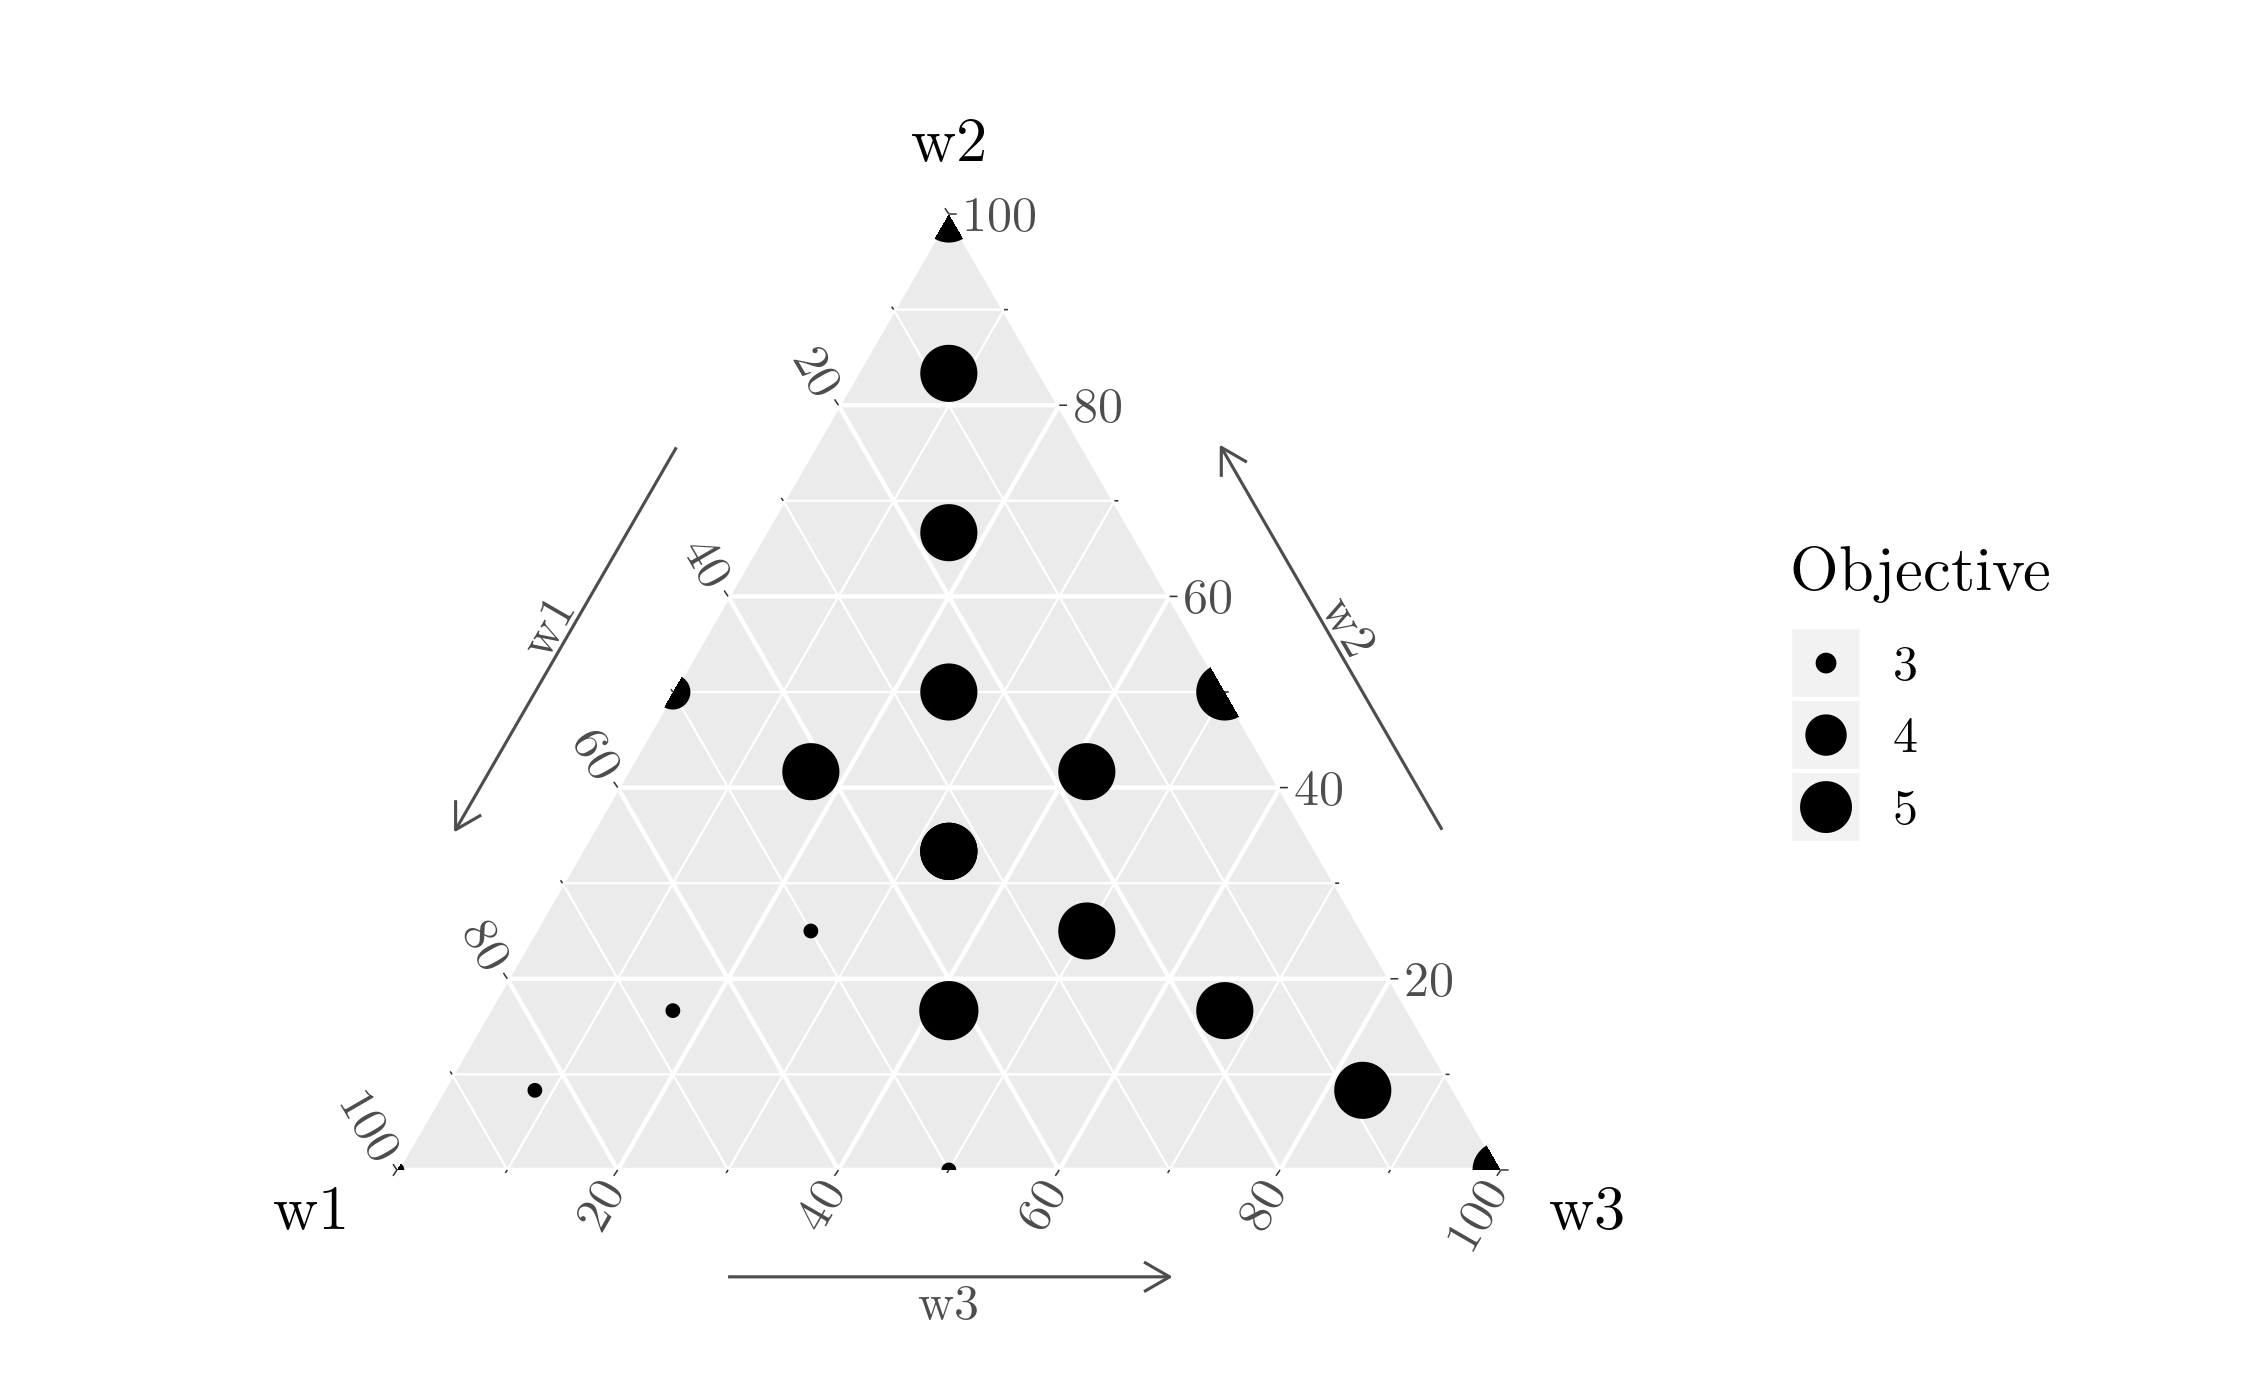
\includegraphics[width=3.5in]{figure/ternary.png}
\DeclareGraphicsExtensions.
\caption{Weight sensitivity ternary plot.}
\label{tern}
\end{figure}

\hypertarget{robust-sense}{%
\subsection{Robustness Analysis}\label{robust-sense}}
The robustness array identified with \(\rho\) was subjected to a sensitivity analysis, therefore a different set of elements where used ranging from \(0\) to \(3\). The graph presented in Figure \ref{rho-permu} identifies the different margin distribution among the three entities. The weights were held constant to a parametrization in suggested by literature.
 
\hypertarget{more-result}{%
  \subsection{More on results: a Lexicographic and Naive comparison}\label{conclusion}}
Because of the lack of any recent research\cite{merville1978} about the topic of Multi-Criteria optimization applied to the field of TP it was worth to set up a rigorous experiment to prove the effectiveness of the robust model. Therefore, the decision was to test the goodness of the model in comparison with two other types of approaches namely:
\begin{itemize}
\item The Naive approach: in this setting, the DM randomly chose one of the possible alternatives for profit allocation in a way that is feasible in the deterministic model;
\item The Lexicographic approach: in such setting the multiobjective problem was set as a Lexicographic Goal Program (LGP), therefore the DM optimized all the objectives in a strict hierarchical order not taking care of possible trade-offs between objectives;
\end{itemize}
The two approaches were compared with the model at its maximum robustness (\emph{i.e.} $\rho=[3,3,3]$), in such setting we could test the feasibility of the results obtained. In the following tables are presented such results. At first sight, it is worth noting from Table \ref{res-comparison} how the allocation changed from one approach to another. In particular, the Lexicographic approach tended to distribute a considerably lower margin through the entities, this behavior is due to the fact that even when deviations are normalized the tax objective tends to shrink the overall profit distribution, such behavior is highlighted also in the weight sensitivity analysis depicted in Figure \ref{tern}. However, a fist overview as proposed in Figure \ref{res-comparison} is not sufficient to highlight the goodness of the robust model. In order to focus more on the characteristics of such model it's worth introducing some more findings especially the ones dealing with the hard constraints, namely:
\begin{itemize}
\item The upper quartile constraint;
\item The lower quartile constraint;
\item The lower bound price constraint;
\item The upper bound price constraint.
\end{itemize}
The last two constraints, namely the one concerning the final price of the good were not involved directly in the process of robustification however the shift in taxes and duties affected indirectly the price (upward shift) therefore making unfeasible some allocations that were not taking into account possible increases in taxes and duties. In Table \ref{fea-comparison} emerges clearly that the allocation as proposed in the previous table is not feasible for the Naive and the Lexicographic approach, in particular, a relatively low shift in the lower quartile can hardly compromise such allocations arising a great amount of TP riskiness. For the Naive approach, the unfeasible points were two, namely: the PLI of the manufacturer that has fallen below the shifted lower quartile and the price of the good that has fallen far above the upper threshold. In case of the Lexicographic approach, the unfeasible points were two, namely: the PLI of the manufacturer that has fallen below the shifted lower quartile and the PLI of the distributor that has fallen below the shifted lower quartile. Leaving aside the considerations about the feasible points, which still remains crucial for the goodness of a TP policy is possible to compare the different objectives achieved by the different approaches by studying the under and over-achievement collected by the deviational variables. The deviational variables were normalized by the goal to be attained in order to allow for a better comparison between each other. In Table \ref{dev-comparison} is possible to notice how the Naive approach tends to accomplish the last two objectives, leaving aside the last tax minimization objective. Conversely, the Lexicographic allowed for greater harmonization of the overall deviation as well as the Robust model, in particular, the Robust model because of the weights allowed for a better trade-off between the management objectives and the compliance objectives imposed by the TP regulations.
\begin{table}[]
\centering
\caption{Results comparison: Robust, Naive and Lexicographic.}
\label{res-comparison}
\begin{tabular}{@{}llll@{}}
\toprule
  Entity       & Robust & Naive & Lexicographic \\ \midrule
  Manufacturer & 1.67   & 1     & 0.99     \\ 
  Distributor  & 1.08   & 2.2   & 0.62     \\
  Principal    & 2.86   & 5.1   & 2.17     \\ \bottomrule
\end{tabular}
\end{table}
\begin{table*}[]
\centering
\caption{Results comparison: feasibility.}
\label{fea-comparison}
\begin{tabular}{@{}llllll@{}}
\toprule
  Indicator         & Robust & Naive & Lexicographic & Lower Bound & Upper Bound \\ \midrule
  Manufacturer PLI  & 0.0680 & 0.0407   & 0.0403     & 0.0460      & 0.1610            \\ 
  Distributor  PLI  & 0.0176 & 0.0359   & 0.0101     & 0.0112      & 0.0560            \\
  Principal    PLI  & 0.0423 & 0.0755   & 0.0321     & 0.0242      & 0.1694            \\ 
  Final Price       & 63.70  & 68.73    & 63.25      & 61.20      & 63.7        \\ \bottomrule
\end{tabular}
\end{table*}
\begin{table*}[]
\centering
\caption{Results comparison: deviations from the objective.}
\label{dev-comparison}
\begin{tabular}{@{}lllllll@{}}
\toprule
  Entity       & \multicolumn{2}{l}{Robust} & \multicolumn{2}{l}{Naive} & \multicolumn{2}{l}{Lexicographic} \\
                        &$\delta^+$&$\delta^-$&$\delta^+$&$\delta^-$&$\delta^+$&$\delta^-$ \\ \midrule
  Tax Objective         & $163.33\%$ & -        & $277.32\%$ & -        & $69.99\%$ & - \\ 
  TNMM Objective        & -         & $97.36\%$ & -          & $6.18\%$ & - & $173.06\%$ \\
  Management Objective  & $49.46\%$  & -        & $25.23\%$  & -        & $65.95\%$ & - \\ \bottomrule
\end{tabular}
\end{table*}
\begin{figure*}[]
\centering
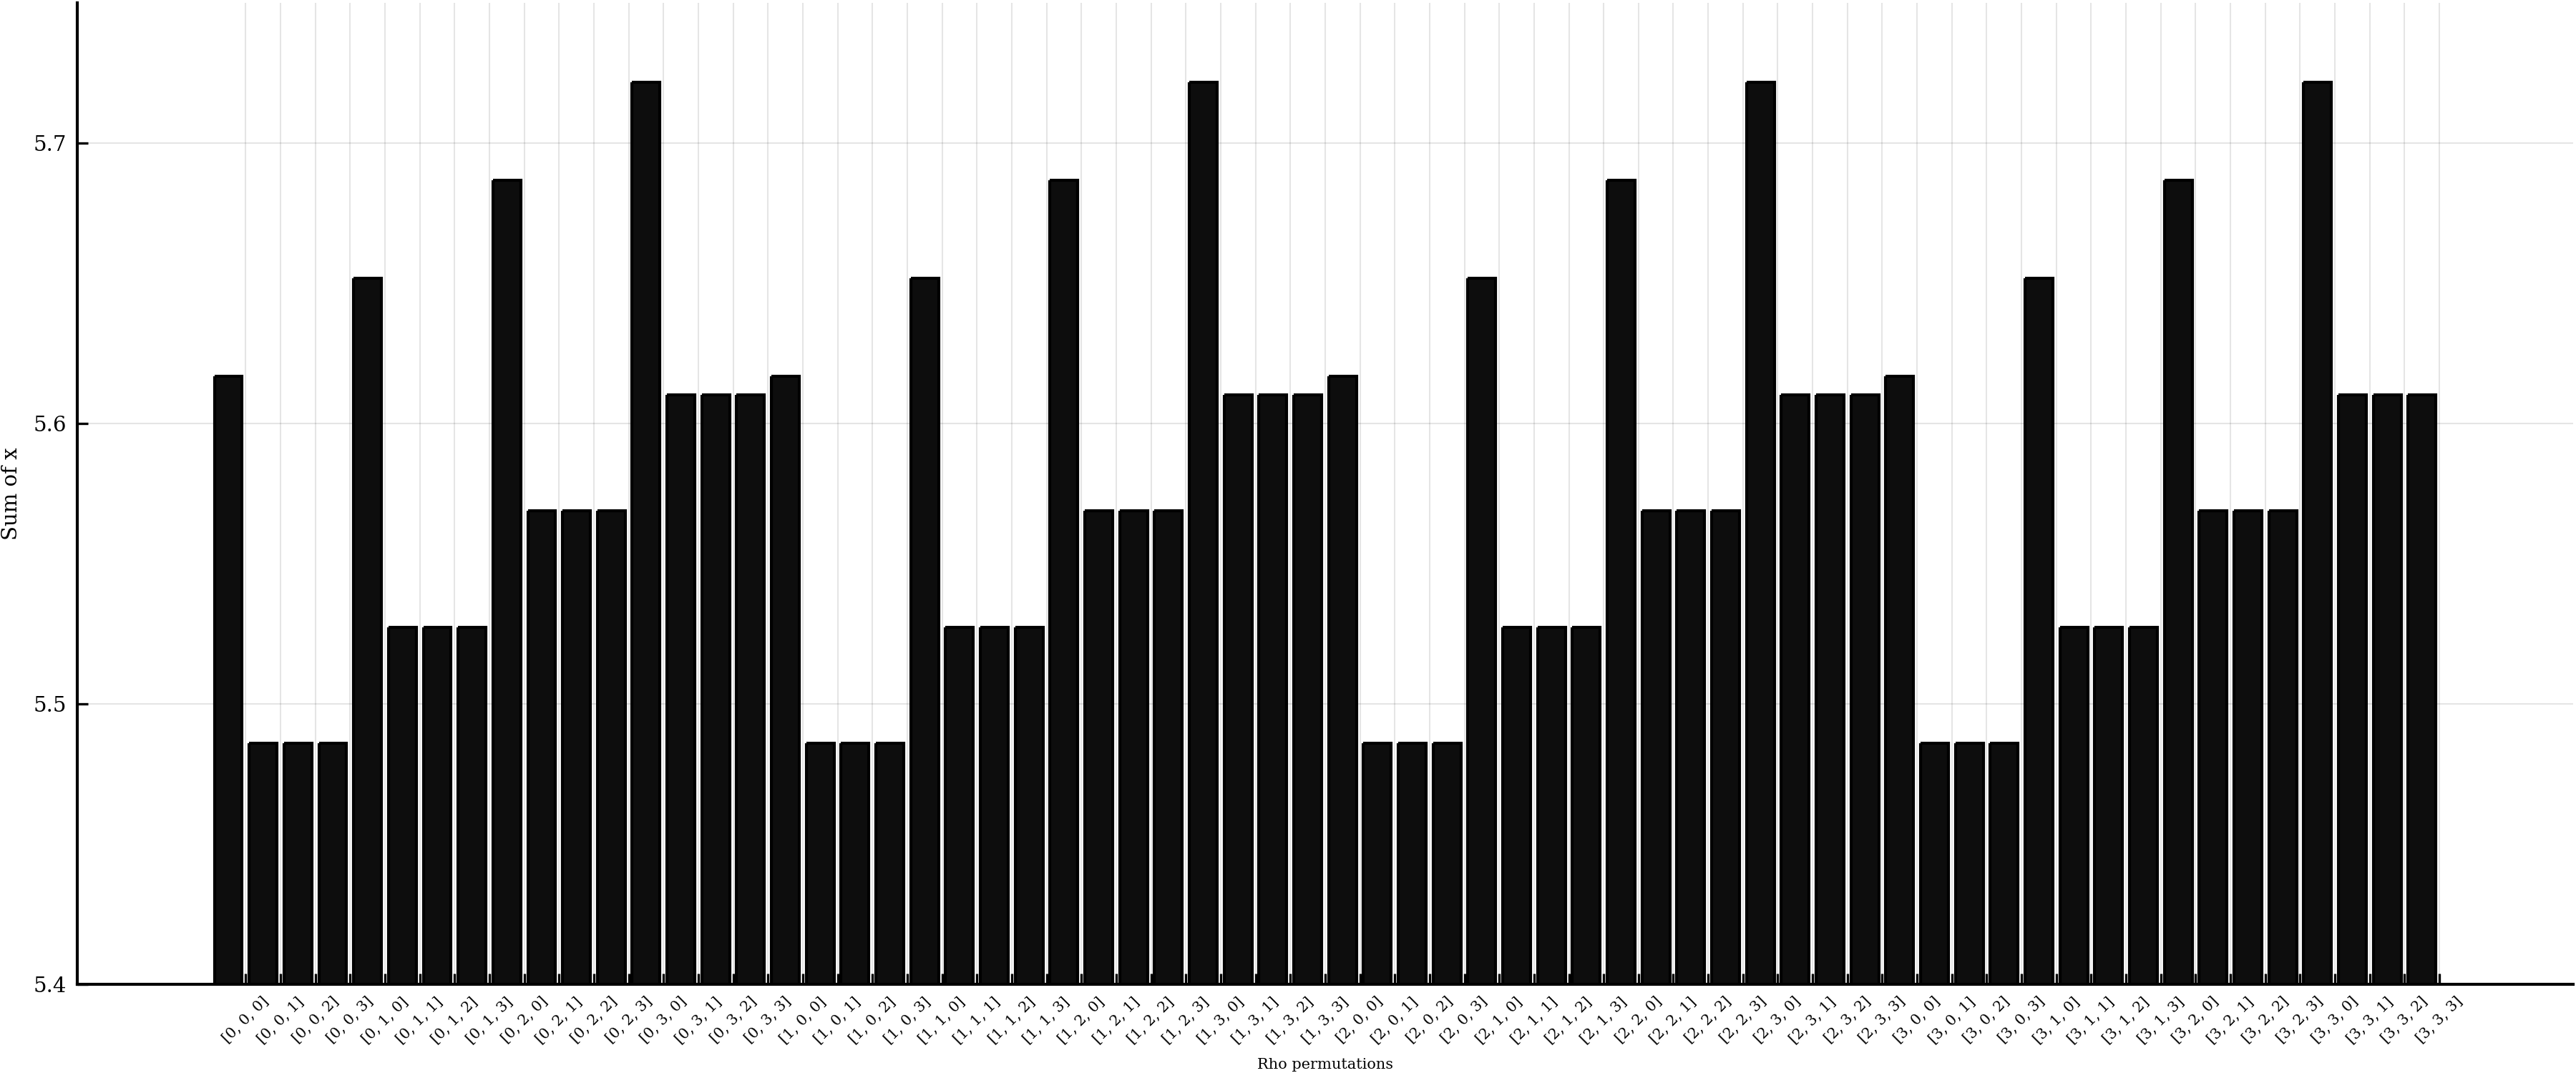
\includegraphics[width=\textwidth]{figure/Figure_1.png}
\DeclareGraphicsExtensions.
\caption{Rho permutations and objective function results.}
\label{rho-permu}
\end{figure*}

\hypertarget{final-results}{%
  \subsection{Final results}\label{conclusion}}
As a last step in table \ref{res-final} are presented the results of the final model in all its main features namely, the DM aspirations embedded through weighting and appropriate satisfaction functions and the uncertainty carried out through specific robust formulation.
\begin{table}[]
\centering
\caption{Final results comparison: model with and without satisfaction function.}
\label{res-final}
\begin{tabular}{@{}lll@{}}
\toprule
  Variable          & No satisfaction function & Satisfaction function \\ \midrule
  $x_1$      & 1.67   & 1.32   \\ 
  $x_2$      & 1.08   & 1.00    \\
  $x_3$      & 2.86   & 1.89     \\\bottomrule
\end{tabular}
\end{table}
 
\hypertarget{conclusion}{%
\section{Conclusion}\label{conclusion}}
The paper proposed a model for intercompany transaction pricing which complies with the legislation in terms of transfer pricing policies. Because of the number of conflicting objectives the best approach seemed to be the GP one. However, taking into account just the conflicting objectives do not leave any remedy to possible uncertainties arising from exogenous variables. Because of that, the concept of RO was introduced. The results were encouraging: the solution remains feasible even in case of shifts of the economic environment and this confirms that the GP in its robust counterpart can indeed be a sounding tool in the hands of professionals when setting their TP policies.

\bibliographystyle{plain} 

\bibliography{reference}

\end{document}

